\documentclass[10pt]{article}
\usepackage[margin=1in]{geometry}
\usepackage{amsmath,graphicx,booktabs,longtable}
\title{Equation (1.27): PINN Evaluation Report}
\author{}\date{}
\begin{document}\maketitle
\noindent\textbf{Run status.} CPU smoke test: pipeline verification only; this is not a trained or validated solution.
\section{Target and scope}
The target is the full nonlinear equation
\[
 iE_t+(1-i\epsilon_1\partial_z)(E_{xx}+E_{yy})-E_{zz}
 -i\epsilon_2E_{zzz}+(1+i\epsilon_1\partial_z)(|E|^2E)=0.
\]
The finite periodic box is a computational approximation, not an assertion of whole-space accuracy. All comparisons below use saved numerical outputs. A Fourier reference must itself pass grid, domain, and time-step checks before it can validate the PINN. The equation's linear weighted-decay estimate is not imposed as a nonlinear decay law.
\section{Field comparison}
The complex-field error includes phase disagreement. Peak and integrated squared-magnitude errors are distinct diagnostics; no phase alignment or renormalization is performed in these comparisons. Reference and PINN use the same evaluation coordinates.
\begin{figure}[!htbp]\centering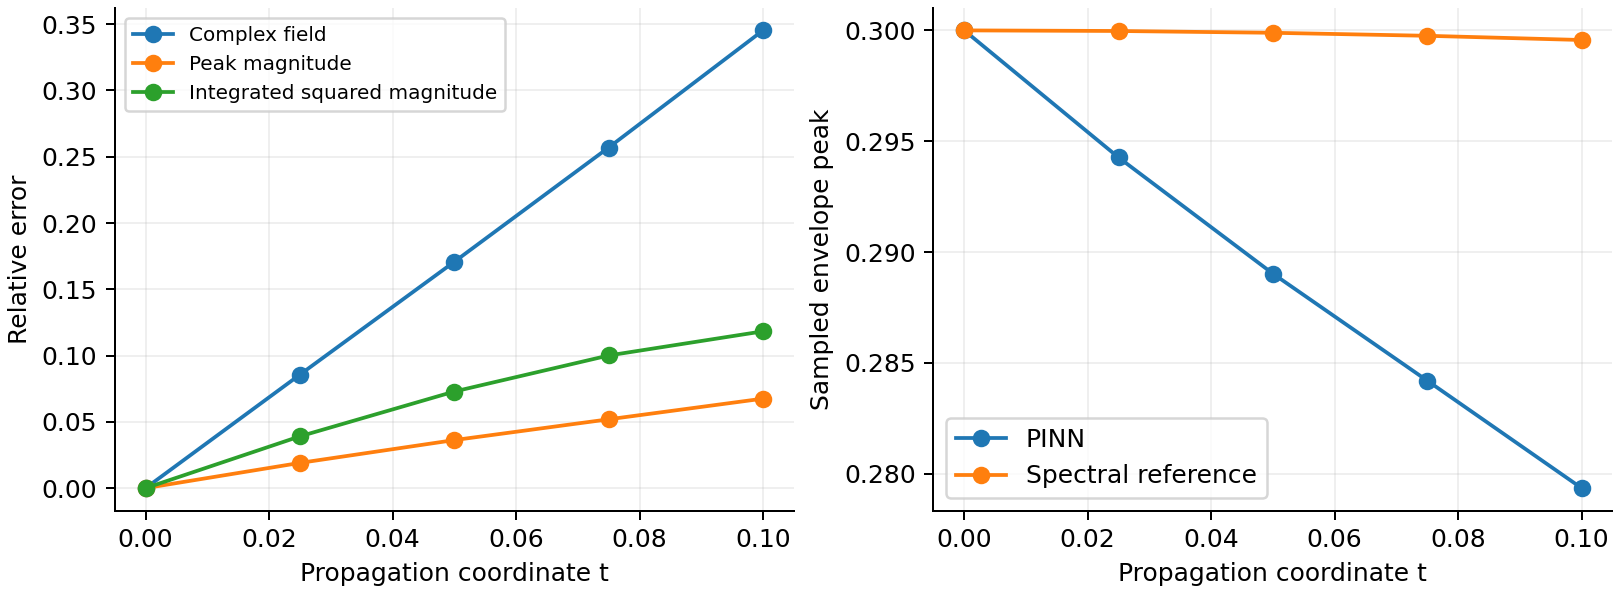
\includegraphics[width=.9\linewidth]{errors.png}
\caption{Measured PINN errors and sampled envelope peaks at the saved evaluation times. A falling predicted peak is not evidence of physical decay if the field errors are large.}\end{figure}
\begin{longtable}{rrrr}\toprule
$t$ & Relative field error & Relative peak error & Relative mass error\\\midrule
0 & 2.548e-16 & 1.85e-16 & 0 \\
0.025 & 0.08564 & 0.01903 & 0.03908 \\
0.05 & 0.1708 & 0.03624 & 0.07287 \\
0.075 & 0.257 & 0.05192 & 0.1001 \\
0.1 & 0.3453 & 0.0675 & 0.1183 \\
\bottomrule\end{longtable}
\clearpage
\section{Spatial structure}
\begin{figure}[!htbp]\centering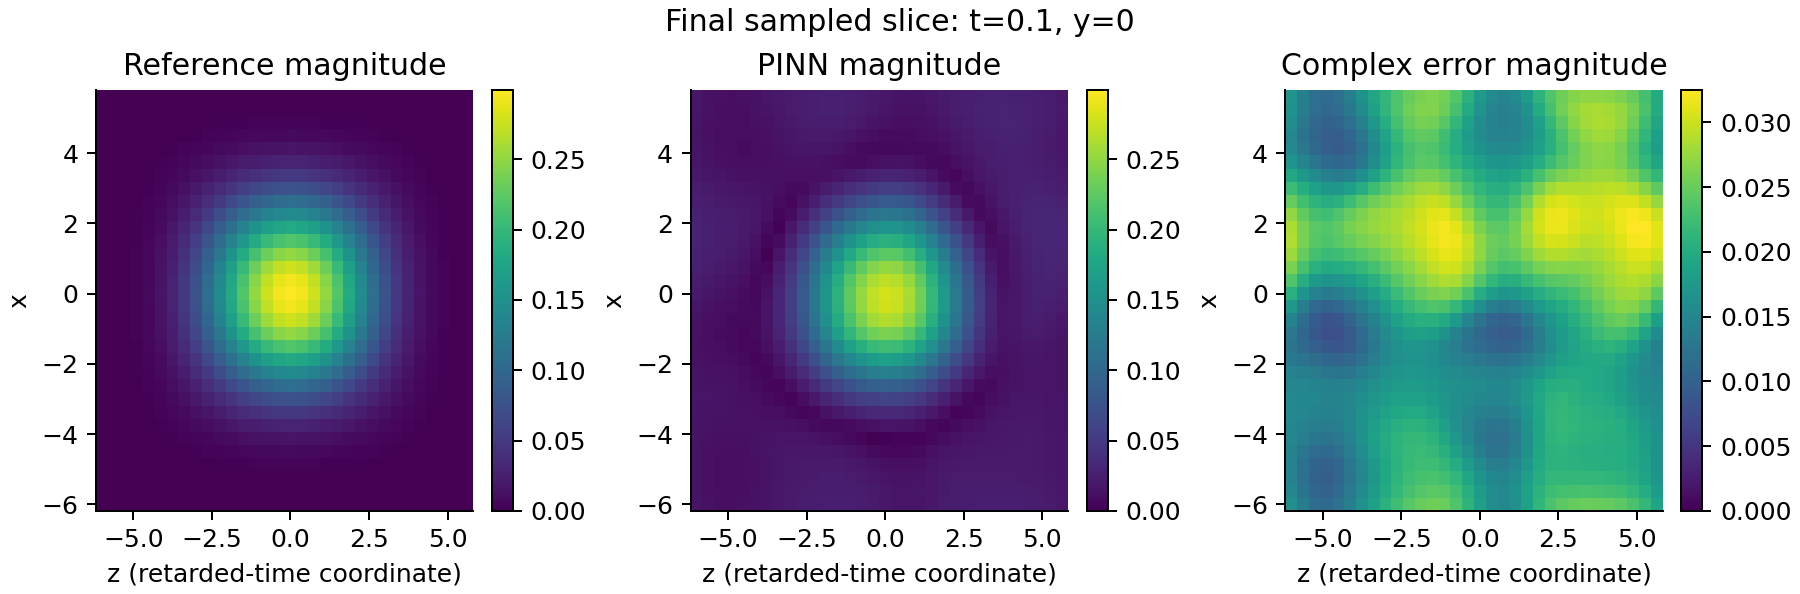
\includegraphics[width=.9\linewidth]{slices.png}
\caption{Final central transverse slice. Reference and prediction magnitudes share one color scale; the complex error has its own scale. The horizontal $z$ axis is the paper's normalized retarded-time coordinate.}\end{figure}
\section{Interpretation and next checks}
A successful smoke run establishes that derivatives, training, checkpointing, reference generation and reporting can execute. It does not establish a useful trained network. Evaluate multiple seeds and points withheld from training; inspect phase and peak errors; refine the reference and evaluate the PDE residual independently. Extend propagation only after short-window reference agreement. For inverse inference of the small coefficients, a separate identifiability and noise study is needed.
\section{Recorded evaluation metadata}
{\small\raggedright\begin{itemize}
\item Configuration: epsilon1=0.00831834509, epsilon2=0.00498719622; T=0.1; periods=[12.0, 12.0, 12.0]; initial amplitude=0.3, trigonometric power=2; dtype=float64.
\item checkpoint\_path: checkpoint.pt
\item reference\_path: reference.npz
\item checkpoint\_sha256: d8a79a57564d8920\allowbreak{}f9791b08734253f2\allowbreak{}5498edc48df53fb7\allowbreak{}9538f10bf9e1a808
\item reference\_sha256: acaa75206deda798\allowbreak{}c19a1a9b985b1d31\allowbreak{}2eff665d784ef70e\allowbreak{}ccabce00fec0f213
\item max\_pinn\_relative\_mass\_drift: 0.11828231009745054
\item max\_reference\_relative\_mass\_drift: 3.2124589401426532e-15
\item equation: Dysthe3D-1.27
\item checkpoint\_step: 5
\item max\_relative\_l2: 0.34532530961149954
\item max\_relative\_peak\_error: 0.06749635660165428
\item max\_mass\_relative\_error: 0.11828231009745338
\item reference\_convergence\_status: not\_\allowbreak{}established\_\allowbreak{}by\_\allowbreak{}this\_\allowbreak{}comparison
\end{itemize}}
The complete machine-readable metrics are supplied alongside this report. The source checkpoint and reference paths identify the inputs; preserve those artifacts and the training configuration for reproducibility.
\end{document}
